%-------------------------------------------------------------
% CV en español
% Hugo Ferrando Seage - 2017
%-------------------------------------------------------------

\documentclass[a4paper, 12pt]{article}
\usepackage[utf8]{inputenc}
\usepackage[T1]{fontenc}
\usepackage[spanish]{babel}
\usepackage{subfig}
\usepackage{tabularx}
\usepackage{paracol}
\usepackage{booktabs}
\usepackage{enumitem} % Customize enumerate items
\usepackage{longtable} % Required to make tables span more than one page
\usepackage{graphicx} % Required for including pictures
\usepackage{multicol}
\usepackage[cm]{fullpage}
\usepackage[usenames,dvipsnames]{xcolor} % Required for specifying custom colors
\usepackage[pdfstartview=Fit]{hyperref} % Required for adding links	and customizing them
\definecolor{linkcolour}{rgb}{0,0.2,0.6} % Link color
\hypersetup{colorlinks,breaklinks,urlcolor=linkcolour,linkcolor=linkcolour, pdfpagemode=UseNone} % Set link colors throughout the document
\hyphenpenalty=10000
\setlength{\columnsep}{-3.5cm}

\newenvironment{myparacol}[2][]{%
\begin{paracol}{#2}[#1]\setlength{\parindent}{0pt}}{%
\end{paracol}}

\begin{document}
\pagestyle{empty} % Removes page numbering

\begin{flushright}
    Graduado en Ingeniería Informática\\
    +34 680 340 463\\
    \href{mailto: me@hugofs.com}{me@hugofs.com}\\
    \href{https://hugofs.com}{hugofs.com}\\
\end{flushright}

\vspace{-27mm} %TODO: Top margin amount

\begin{figure}[ht!]
    \begin{flushleft}
        \subfloat{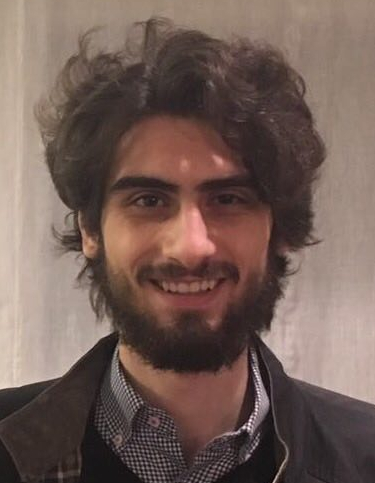
\includegraphics[width=0.13\textwidth]{hugo.jpg}}
    \end{flushleft}
\end{figure}

{\textsc {\Huge \vspace{5mm} \hspace{-13mm} Hugo Ferrando Seage}}\\

\setlength{\columnsep}{24pt}
\begin{sloppypar}
\begin{myparacol}{2}
    EDUCACIÓN
    \vspace{1mm}
    \hrule
    \kern9pt
    \textbf{U-tad} \hfill 17 --- 18

    Máster en Computación Gráfica y Simulación\\

    \textbf{Universidad Europea de Madrid} \hfill 14 --- 17

    Grado en Ingeniería Informática

    \textit{TFG:} \href{https://github.com/hugo19941994/movie-pepper-doc/raw/master/thesis.pdf}{Estudio sobre sistemas de recomendación de películas basados en el procesamiento de lenguaje natural}

    \textit{Actividades:} Club de Robótica, Data Science Lab

    \textit{Media:} 7.8/10\\

    \textbf{Univ. Politécnica de Madrid} \hfill 12 --- 14

    Grado en Ingeniería Informática

    \textit{Actividades:} Capítulo de Estudiantes ACM
    \\

    \switchcolumn{}

    EXPERIENCIA
    \vspace{1mm}
    \hrule
    \kern9pt

    \textbf{Telefónica I+D} \hfill dec 17 ---

    Ingeniero de Software en SmartDigits\\

    \textbf{Telefónica $\sim$ Talentum} \hfill sep 16 --- nov 17

    Proyectos en Telefónica I+D \& LUCA

    Mejoras del sistema de recomendación content-to-content de Movistar+\\

    \textbf{Product Hackers} \hfill jun 16 --- oct 16

    Desarrollo de web apps y chat bots usando Ionic y Angular 2 para móviles y web\\

    \textbf{UEM} \hfill sep 15 --- mar 17

    \href{https://www.researchgate.net/publication/314142014_Prediction_of_User_Opinion_for_Products_-_A_Bag-of-Words_and_Collaborative_Filtering_based_Approach}{Modelo de predicción de gustos de usuarios a partir de textos de opinión en Amazon, usando Apache Spark}

    Detección de personas en piscinas y playas usando OpenCV para un dron salvavidas

    \href{https://github.com/hugo19941994/infrac-coche}{App para detectar, alertar y registrar infracciones de tráfico usando OpenCV en Android}
    \\

    \switchcolumn{}

    CONOCIMIENTOS TÉCNICOS
    \vspace{1mm}
    \hrule
    \kern9pt

    Python, C++, Go, Javascript ES7, Bash\\

    Apache Spark, React, Angular, Flask, OpenGL, Android SDK \& NDK\\

    GNU/Linux, Git, SSH, GPG, \LaTeX, Markdown, Nginx, Jenkins\\

    IDIOMAS
    \vspace{1mm}
    \hrule
    \kern9pt
    \noindent\begin{tabularx}{\columnwidth}{ @{} X X X }
        Español & Inglés & Italiano
    \end{tabularx}
    \\

    CERTIFICACIONES
    \vspace{1mm}
    \hrule
    \kern9pt
    Certificate in Advanced English (CAE)

    CCNA 1: Introduction to Networks

    CCNA 2: Routing and Switching Essentials

    CCNA 4: Connecting Networks

    \switchcolumn{}

    \noindent PROYECTOS
    \vspace{1mm}
    \hrule
    \kern9pt
    \href{https://github.com/hugo19941994/space-invaders-emu}{Space Invaders emulator}: Emulador de Space Invaders para OSX hecho con C++ y OpenGL

    \href{https://github.com/hugo19941994/chip8-emu}{CHIP8 emulator}: Emulador de CHIP-8 para Windows y Linux

    \href{https://vpn.hugofs.com}{ovpn}: Proveedor de VPN basadas en OpenVPN

    \href{https://github.com/hugo19941994/ViajeFacil}{ViajeFácil}: Software de gestión para agencias de vuelos

    \href{https://github.com/hugo19941994/cv-parser}{CV Parser}: Sistema para gestionar CV usando reconocimiento de entidades nombradas y redes bayesianas

    \href{https://github.com/hugo19941994/robot}{Human Rescue Bot}: Ganador del Laureate Awards for Excellence in Robotics Engineering 2016

\end{myparacol}
\end{sloppypar}
\end{document}
